

%%%%%%%%%%%%%%%%%%%%%%%%%%%%%%%%%%%%%%%%%%%%%%%%%%%%%%%%%%%%%%%%%%%%%%%%%%
%%%%%%%%%%%%%%%%%%%%%%%%%%%%%%%%%%%%%%%%%%%%%%%%%%%%%%%%%%%%%%%%%%%%%%%%%%
\begin{frame}
  \begin{small}
              
  \begin{columns}
  \column{0.9\textwidth}
  {\cb Intergovernmental Panel on Climate Change (IPCC) Assessment Report 6 (2021)}
    \begin{itemize}\setlength\itemsep{1.0ex}\footnotesize
      \item[o]  \hhref{https://www.ipcc.ch/report/ar6/wg3/downloads/report/IPCC_AR6_WGIII_SPM.pdf}{Working Group III:  Mitigation of Climate Change}
    \end{itemize}
  \end{columns}

  \end{small}
\end{frame}   

%%%%%%%%%%%%%%%%%%%%%%%%%%%%%%%%%%%%%%%%%%%%%%%%%%%%%%%%%%%%%%%%%%%%%%%%%%%%%%%%%%
\begin{frame}
  \frametitle{\centerline{\hhref{https://www.ipcc.ch/report/ar6/wg3/downloads/report/IPCC_AR6_WGIII_SPM.pdf}{IPCC  Mitigation of Climate Change:} Growth in anthropogenic greenhouse gas emissions}}
  \begin{scriptsize}

    \begin{columns}
      \column{1.0\textwidth}
      \begin{itemize}\setlength\itemsep{1.9ex}
        \item[o] Aggregate annual global net anthropogenic emissions for major groups of greenhouse gas gases from 1990 to 2019, reported in equivalent gigatonnes of CO$_2$ based on global warming potentials. Growth in anthropogenic emissions has persisted across all major groups of greenhouse gasses since 1990. By 2019, the largest growth in absolute CO$_2$ equivalent emissions was from fossil fuels and industry, followed by methane. The single-year peak of emissions in 1997 was due to higher CO$_2$ equivalent emissions from a forest and peat fire event in South East Asia.

        \item[o] {\it Net anthropogenic greenhouse gas emissions have increased since 2010 across all major sectors globally.} An increasing share of emissions can be attributed to urban areas. Emissions reductions in CO$_2$ from fossil fuels and industrial processes, due to improvements in energy intensity of GDP and carbon intensity of energy, have been less than emissions increases from rising global activity levels in industry, energy supply, transport, agriculture and buildings (high confidence).

      \end{itemize}

    \end{columns}

    \vspace{-0.1cm}
    \begin{columns}
      \column{0.99\textwidth}
      \begin{center}
          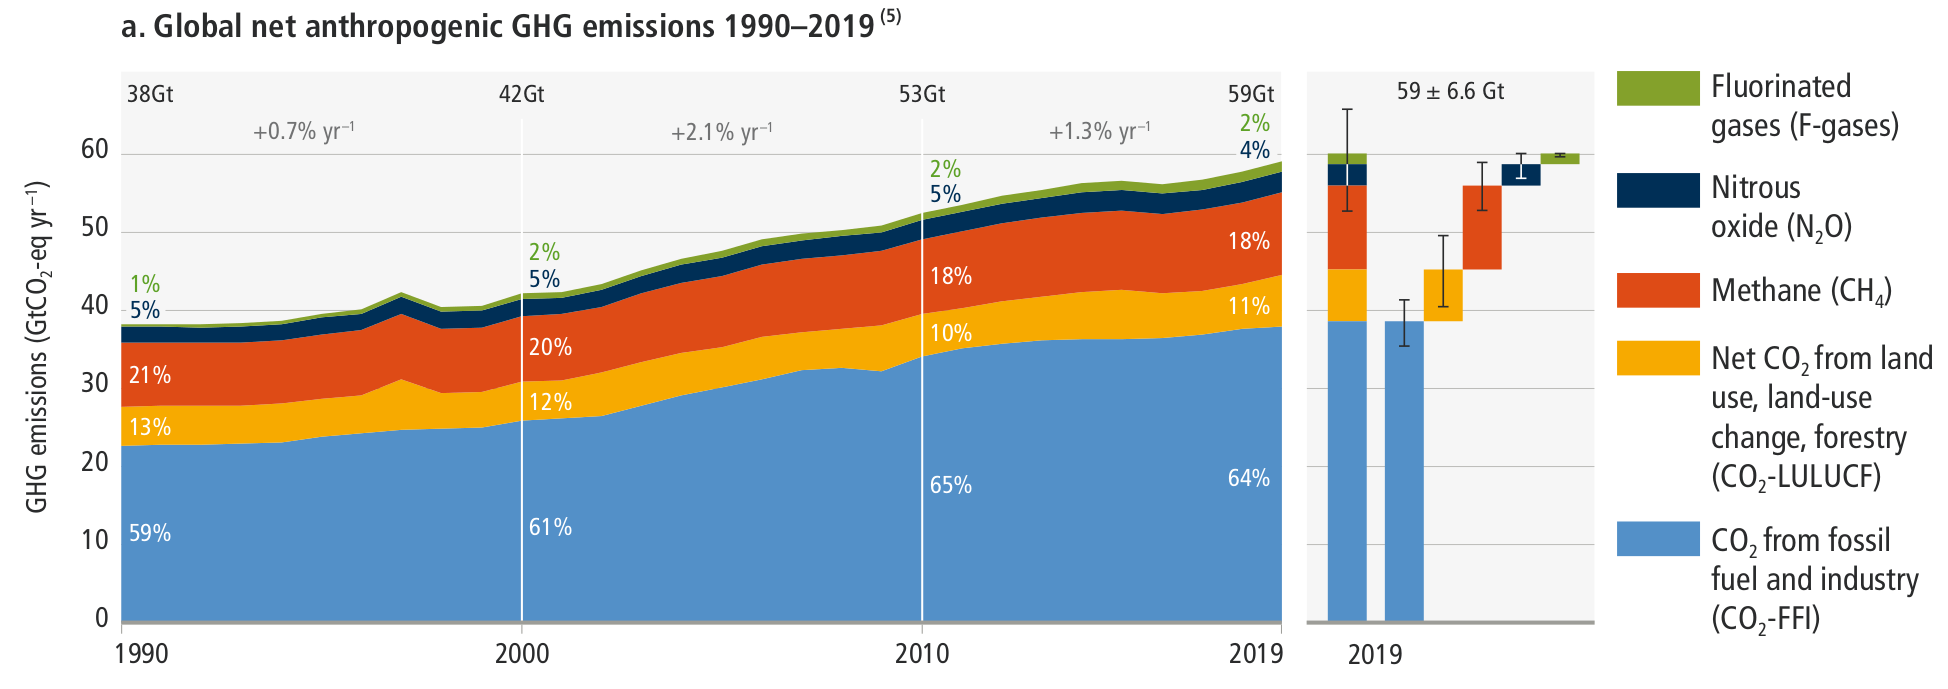
\includegraphics[width=1.0\textwidth]{plots/WG3_net_greenhouse_emissions.png}
      \end{center}   
    \end{columns}

  \end{scriptsize}
  \end{frame} 

%%%%%%%%%%%%%%%%%%%%%%%%%%%%%%%%%%%%%%%%%%%%%%%%%%%%%%%%%%%%%%%%%%%%%%%%%%%%%%%%%%
\begin{frame}
  \begin{scriptsize}

    \vspace{-0.1cm}
    \begin{columns}
      \column{0.43\textwidth}
      \begin{center}
          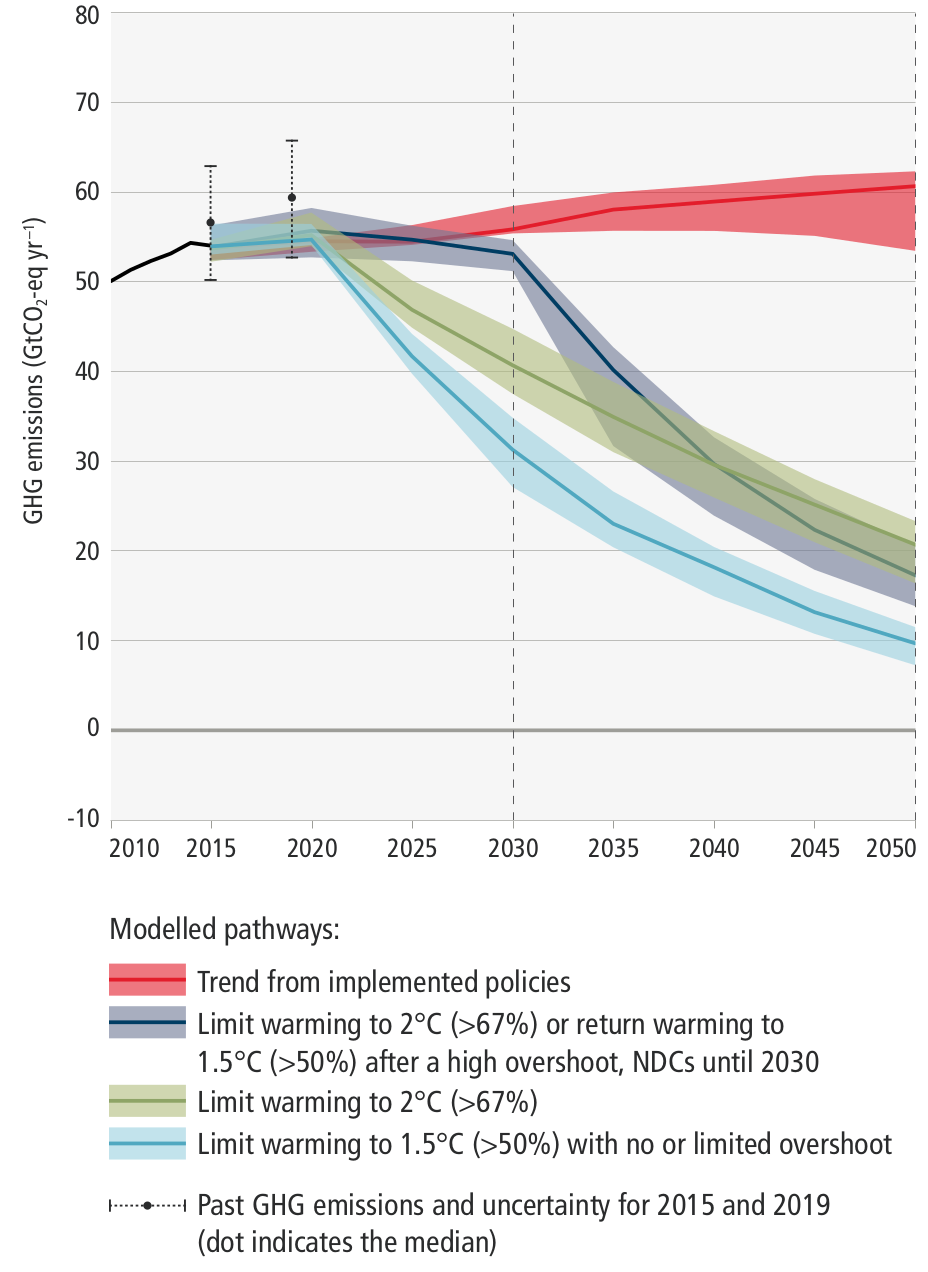
\includegraphics[width=1.0\textwidth]{plots/WG3_global_GHG_emissions.png}
      \end{center}  
      
      \column{0.5\textwidth}
      \hhref{https://www.ipcc.ch/report/ar6/wg3/downloads/report/IPCC_AR6_WGIII_SPM.pdf}{IPCC  Mitigation of Climate Change}

      \begin{itemize}\setlength\itemsep{1.9ex}        
        \item[o] Predicted global greenhouse emissions in 2030 associated with the implementation of Nationally Determined
        Contributions announced prior to the 2021 United Nations Climate Change Conference (COP26) would make it likely that warming will exceed 1.5$^\circ$C during the 21st century. Policies implemented by the end of 2020 are projected to result in higher global greenhouse gas emissions than those implied by NDCs, indicating an implementation gap.

        \item[o]  Attempting to limit warming to below 2$^\circ$C would then rely on a rapid acceleration of mitigation efforts after 2030. Continued investments in unabated high-emitting infrastructure and limited development and deployment of low-emitting
        alternatives prior to 2030 would act as barriers to this acceleration and increase risks of failing to meet the  2$^\circ$C goal.

        \item[o] Reducing greenhouse gas emissions across the full energy sector requires major transitions, including a substantial reduction in overall fossil fuel use, the deployment of low-emission energy sources, switching to alternative energy carriers, and energy efficiency and conservation. The continued installation of unabated fossil fuel infrastructure will 'lock-in' \hhref{https://www.theguardian.com/environment/ng-interactive/2022/may/11/fossil-fuel-carbon-bombs-climate-breakdown-oil-gas}{future emissions}.
      \end{itemize}

    \end{columns}

  \end{scriptsize}
  \end{frame}   
  
%%%%%%%%%%%%%%%%%%%%%%%%%%%%%%%%%%%%%%%%%%%%%%%%%%%%%%%%%%%%%%%%%%%%%%%%%%%%%%%%%%
\begin{frame}
  \begin{scriptsize}

    \vspace{-0.1cm}
    \begin{columns}
      \column{0.52\textwidth}
      \begin{center}
          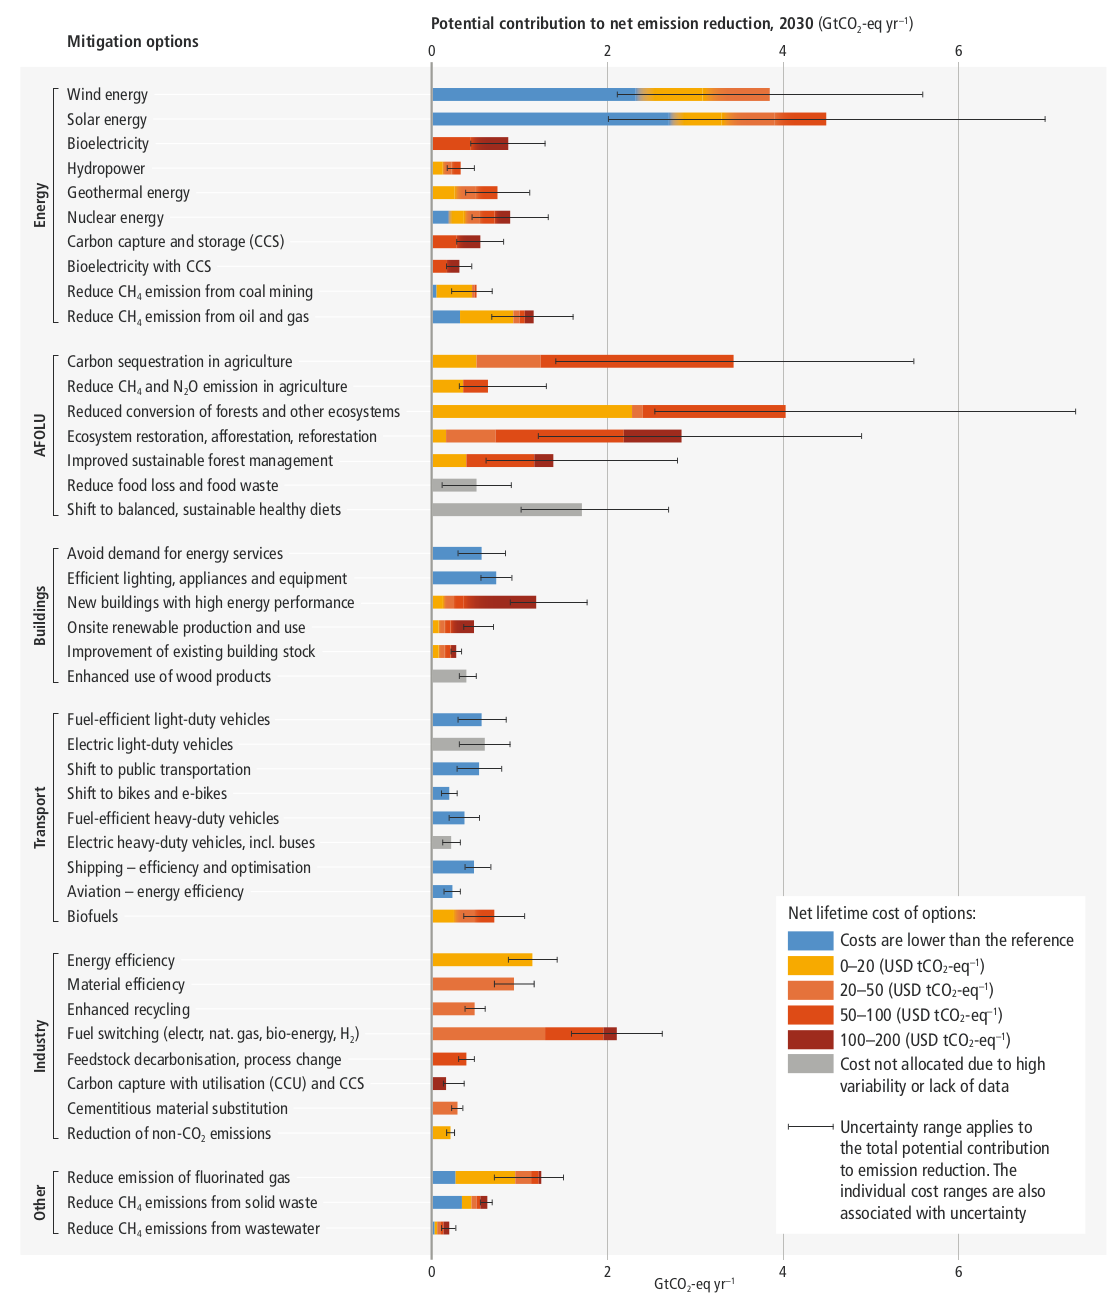
\includegraphics[width=1.0\textwidth]{plots/WG3_mitigation_options.png}
      \end{center}   

      \column{0.4\textwidth}
      \hhref{https://www.ipcc.ch/report/ar6/wg3/downloads/report/IPCC_AR6_WGIII_SPM.pdf}{IPCC  Mitigation of Climate Change}
      \begin{itemize}\setlength\itemsep{1.9ex}        

        \item[o] Estimates of aggregate economic benefits from avoiding damages from climate change (and from reduced climate adaptation costs) increase with the stringency of mitigation. Models that incorporate the economic damages from climate change find that the global economic benefits of reducing warming are greater than the global cost of limiting warming to 2$^\circ$C over the 21st century.

        \item[o] All global modelled pathways that limit warming to 1.5$^\circ$C with no or limited overshoot, and those that limit warming to 2$^\circ$C, involve deep and rapid (and in most cases immediate) greenhouse gas emission reductions in all sectors. 
        
        \item[o] Modelled mitigation strategies to achieve these reductions include transitioning from fossil fuels to very low- or zero-carbon energy sources, such as renewables, or transitioning to fossil fuels with carbon capture and storage. Additional strategies require reducing energy demand and consumption, improving efficiency, reducing non-CO$_2$ emissions, and deploying CO$_2$ removal methods to counterbalance residual emissions.

      \end{itemize}

    \end{columns}

  \end{scriptsize}
  \end{frame} 

%%%%%%%%%%%%%%%%%%%%%%%%%%%%%%%%%%%%%%%%%%%%%%%%%%%%%%%%%%%%%%%%%%%%%%%%%%%%%%%%%%
\begin{frame}
  \begin{scriptsize}
              
  \vspace{-0.1cm}
  \begin{columns}
    \column{0.25\textwidth}
   Sources of CO$_2$ emissions in France:\\
   \vspace{0.1cm} 
   \hhref{https://rustem.web.cern.ch/climate/LeMondeClimateEmergencyFranceImpact.pdf}{Le Monde, May 30th, 2022}

    \column{0.55\textwidth}
    \begin{center}
        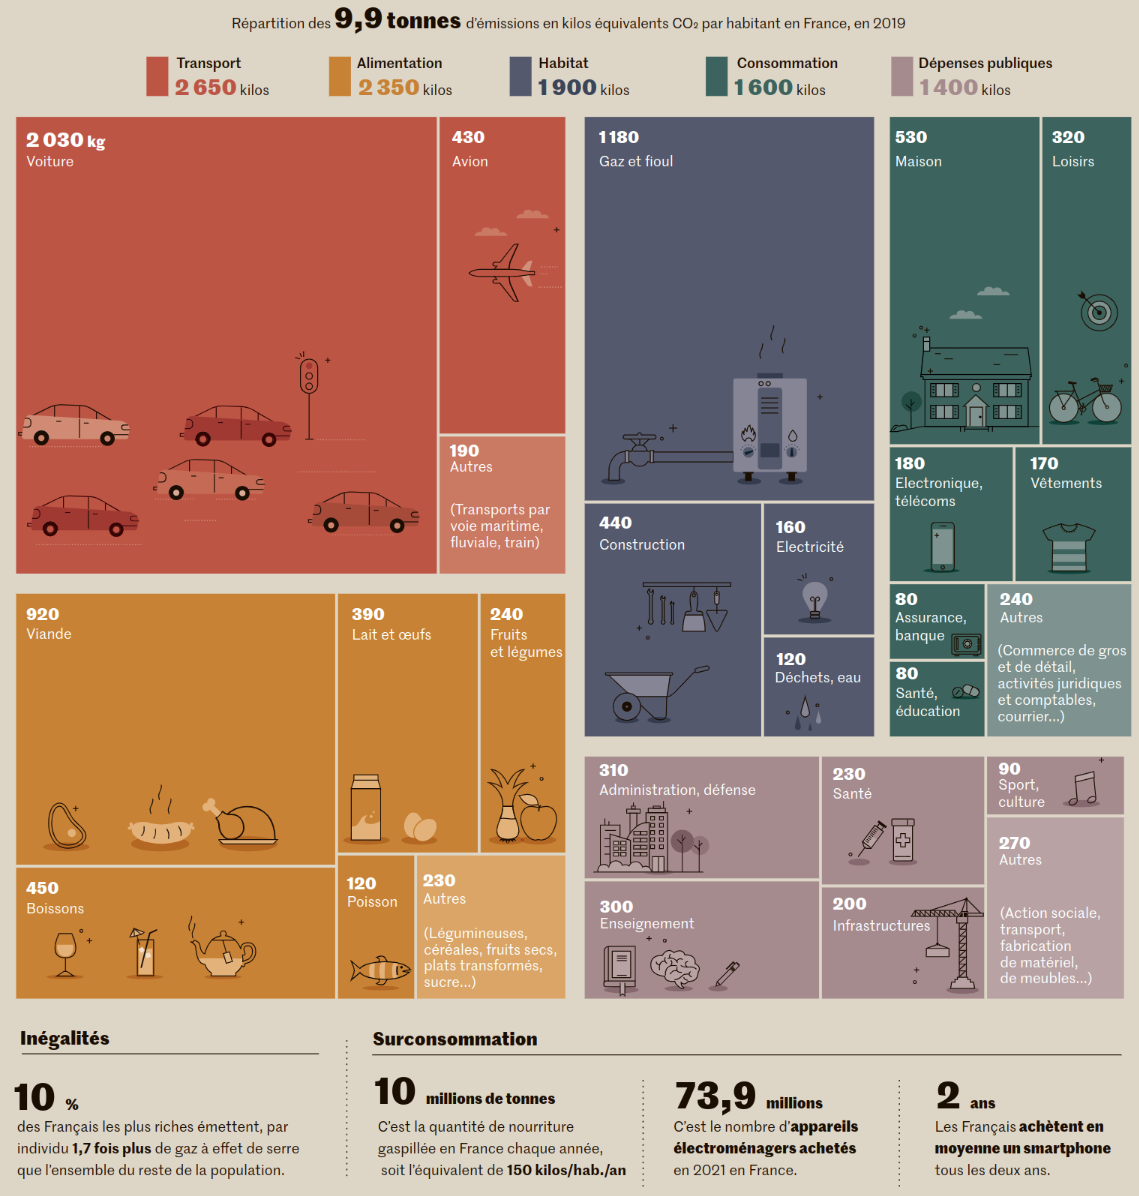
\includegraphics[width=1.0\textwidth]{plots/co2_breakdown.png}
    \end{center}
  \end{columns}

  \end{scriptsize}
  \end{frame}